%%%%%%%%%%%%%%%%%%%%%%%%%%%%%%%%%%%%%%%%%%%%%%%%%%%%%%%%%%%%%%%%%%%%%%
% LaTeX Template: Project Titlepage
%
% Source: http://www.howtotex.com
% Date: April 2011
% 
% This is a title page template which be used for articles & reports.
% 
% Feel free to distribute this example, but please keep the referral
% to howtotex.com
% 
%%%%%%%%%%%%%%%%%%%%%%%%%%%%%%%%%%%%%%%%%%%%%%%%%%%%%%%%%%%%%%%%%%%%%%
% How to use writeLaTeX: 
%s
% You edit the source code here on the left, and the preview on the
% right shows you the result within a few seconds.
%
% Bookmark this page and share the URL with your co-authors. They can
% edit at the same time!
%
% You can upload figures, bibliographies, custom classes and
% styles using the files menu.
%
% If you're new to LaTeX, the wikibook is a great place to start:
% http://en.wikibooks.org/wiki/LaTeX
%
%%%%%%%%%%%%%%%%%%%%%%%%%%%%%%%%%%%%%%%%%%%%%%%%%%%%%%%%%%%%%%%%%%%%%%
%
% --------------------------------------------------------------------
% Preamble
% --------------------------------------------------------------------
\documentclass[paper=a4, fontsize=10pt]{scrartcl}	% KOMA
\usepackage[bottom=1.1in, top=0.9in]{geometry}
\usepackage{lmodern}

\newcommand{\specialcell}[2][c]{%
	\begin{tabular}[#1]{@{}c@{}}#2\end{tabular}}
\usepackage{todonotes}
\usepackage{listings}
\usepackage{graphbox}
\usepackage{hyperref}
\usepackage{twoopt}
\usepackage{adjustbox}
\usepackage[english]{babel}
\usepackage{graphicx}
\usepackage{subcaption}
\usepackage{pgfplots}
\usepackage{mwe}
\usepackage{color, colortbl}
\usepackage[protrusion=true,expansion=true]{microtype}	
\usepackage{amsmath,amsfonts,amsthm,amssymb}
\usepackage{tabularx}
\usepackage{float}

\usepackage{lmodern}
\usepackage{amsmath}
\usepackage{todonotes}
\usepackage{listings}
\usepackage{graphbox}
\usepackage{hyperref}
\usepackage{twoopt}
\usepackage{adjustbox}
\usepackage[english]{babel}
\usepackage{graphicx}
\usepackage{subcaption}
\usepackage{mwe}
\usepackage{color, colortbl}
\usepackage[protrusion=true,expansion=true]{microtype}	
\usepackage{amsmath,amsfonts,amsthm,amssymb}
\usepackage{tabularx}
\usepackage{float}
\usepackage{tikz} 
\usepackage{xcolor}
\usepackage{listings}
\usepackage{arydshln}
\usepackage{bytefield}

\definecolor{mGreen}{rgb}{0,0.6,0}
\definecolor{mGray}{rgb}{0.5,0.5,0.5}
\definecolor{mPurple}{rgb}{0.58,0,0.82}
\definecolor{backgroundColour}{rgb}{0.95,0.95,0.92}

\newcommand\setrow[1]{\gdef\rowmac{#1}#1\ignorespaces}
\newcommand\clearrow{\global\let\rowmac\relax}
\usepackage{graphicx}
\usepackage[T1]{fontenc}
\definecolor{Red}{rgb}{1,0.7,0.7}
\definecolor{Yellow}{HTML}{FAFAD2}
\definecolor{Green}{HTML}{9ACD32}
\definecolor{Blue}{rgb}{0.5,0.8,1}
\lstset{
	frame=single,
	xleftmargin=15pt,
	xrightmargin=15pt,
	basicstyle=\ttfamily\small
}
\lstdefinestyle{CStyle}{
	backgroundcolor=\color{backgroundColour},   
	commentstyle=\color{mGreen},
	keywordstyle=\color{magenta},
	numberstyle=\tiny\color{mGray},
	stringstyle=\color{mPurple},
	basicstyle=\footnotesize,
	breakatwhitespace=false,         
	breaklines=false,                 
	captionpos=b,                    
	keepspaces=true,                 
	numbers=left,                    
	numbersep=5pt,                  
	showspaces=false,                
	showstringspaces=false,
	showtabs=false,                  
	tabsize=2,
	language=C
}
\lstset{basicstyle=\ttfamily,
	showstringspaces=false,
	commentstyle=\color{red},
	keywordstyle=\color{blue}
}


\usepackage{graphicx}
\usepackage[T1]{fontenc}
\definecolor{Red}{rgb}{1,0.7,0.7}
\definecolor{Yellow}{HTML}{FAFAD2}
\definecolor{Green}{HTML}{9ACD32}
\definecolor{Blue}{rgb}{0.5,0.8,1}
\lstset{
	backgroundcolor=\color{backgroundColour},   
	commentstyle=\color{mGreen},
	keywordstyle=\color{magenta},
	numberstyle=\tiny\color{mGray},
	stringstyle=\color{mPurple},
	basicstyle=\footnotesize,
	breakatwhitespace=false,         
	breaklines=false,                 
	captionpos=b,                    
	keepspaces=true,                 
	numbers=left,                    
	numbersep=5pt,                  
	showspaces=false,                
	showstringspaces=false,
	showtabs=false,                  
	tabsize=2,
	frame=single,
	xleftmargin=15pt,
	xrightmargin=15pt,
	basicstyle=\ttfamily\small
}
% --------------------------------------------------------------------
% Definitions (do not change this)
% --------------------------------------------------------------------
\newcommand{\HRule}[1]{\rule{\linewidth}{#1}} 	% Horizontal rule
\newcommandtwoopt*{\myref}[3][][]{%
	\hyperref[{#3}]{%
		\ifx\\#1\\%
		\else
		#1~%
		\fi
		\ref*{#3}%
		\ifx\\#2\\%
		\else
		\,#2%
		\fi
	}%
}

\makeatletter							% Title
\def\printtitle{%						
	{\centering \@title\par}}
\makeatother									

\makeatletter							% Author
\def\printauthor{%					
	{\centering \large \@author}}				
\makeatother							

% --------------------------------------------------------------------
% Metadata (Change this)
% --------------------------------------------------------------------
\title{	\normalsize \textsc{Politecnico di Torino\\GPU Programming} 	% Subtitle
	\\[2.0cm]								% 2cm spacing
	\HRule{0.5pt} \\						% Upper rule
	\LARGE \textbf{\uppercase{Assignment:\\CUDA Video Streaming}}	% Title
	\HRule{2pt} \\ [0.5cm]		% Lower rule + 0.5cm spacing
	\normalsize 
	\today % Todays date
}

\author{
	Group 16
}

\begin{document}
	% ------------------------------------------------------------------------------
	% Maketitle
	% ------------------------------------------------------------------------------
	\thispagestyle{empty}		% Remove page numbering on this page
	
	\printtitle					% Print the title data as defined above
	\vfill
	\printauthor				% Print the author data as defined above
	\newpage
	% ------------------------------------------------------------------------------
	% Begin document
	% ------------------------------------------------------------------------------
	\setcounter{page}{1}		% Set page numbering to begin on this page

	\section{HeatMap}
	Since the basis of this project is to send the pixel difference, the lower the dissimilarities the higher the bandwidth saving. In order to better visualize which pixels changes the most and the different magnitudes, an heatmap is generated with the current and the previous frames.\newline\newline	
	A heat map is nothing else than a data visualization technique that represents the magnitude of a measurement as colors in two dimensions, in this case an image. The idea is first compute the difference at the pixel level between two successive frames and then represent it using a color scale from blue to red, where blue means low difference and red high difference. The Image \ref{fig:heat_v0} shows a naif implementation of heat map, available at \texttt{heat\_map\_benchmark/v0.cu}, that generates in real time the image on the right.

	\begin{figure}[H]
		\centering
		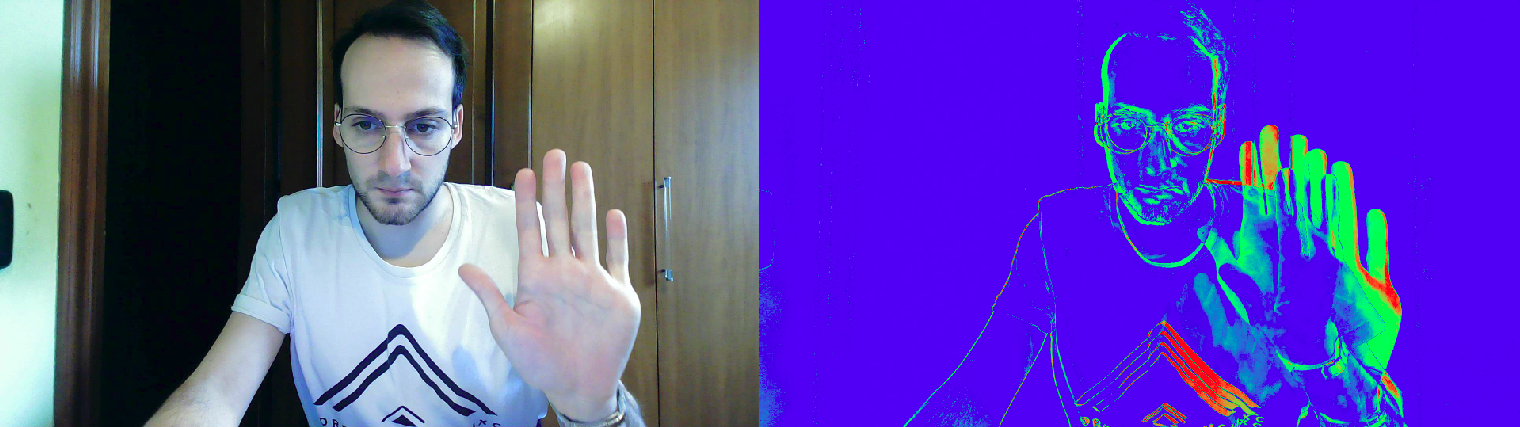
\includegraphics[width=0.9\linewidth]{images/heatmap/v0}
		\caption{\textit{Example of real-time heat map from webcam}}
		\label{fig:heat_v0}
	\end{figure}
	The basic steps for generating an heat map are the following:
	\begin{itemize}
		\itemsep0sp
		\item Take two frames from the webcam via OpenCV
		\item Compute the pixel difference
		\item Translate the difference into the corresponding color for the heat map
		\item Copy the result into a support buffer image and visualize it
	\end{itemize}
	All programs versions for the heat map are available in the \texttt{heat\_map\_benchmark} folder.
	
	\subsection{Heat map pixel mapping - CPU Naif implementation}
	
	The first \textit{naif} version has been done on the CPU. This implementation can generate an heatmap in more or less 980ms, that is too much. This is also due to the complexity of the function itself that is used to map a normalized pixel difference to a blue-red scale and because the image is sequentially analyzed.
	In order to convert the difference of a pixel into the three color component (RGB), the usage of the \textit{sine} function has been done. The difference of the each pixel has been computed as the sum of the absolute value of the difference of the single color component, as:
	\[
		diff = abs(Previous[i,R] - Curr[i,R]) + abs(Previous[i,G] - Curr[i,G] + abs(Previous[i,B] - Curr[i,B])
	\]
	Where $Previous[i,R]$ is the pixel red color component of the pixel at index $i$. In the worst case, a pixel can be turned from black to white or vice versa and so, the $0 \leq diff \leq 765$, that is $255 \cdot 3$. Then the $diff$ value is taken and normalize, by using 765 so that, $0 \leq diff_{norm} \leq 1$.:
	\[
		diff_{norm} = \frac{diff}{765}
	\]
	
	This value must be mapped into the tree RGB component of the heat map; the pixel must be more blue if the difference is more toward 0.0, yellow/green if near 0.5 and red if next to 1.0.
	The smoothed way to perform this task is to use three different sine functions, centered respectively on 0.0, 0.5 and 1.0 as in the following way:
	\begin{align*}
		\text{RED    } & \quad sin(\pi \cdot diff_{norm} - \frac{\pi}{2.0})\\
		\text{GREEN  } & \quad sin(\pi \cdot diff_{norm})\\
		\text{BLUE   } & \quad sin(\pi \cdot diff_{norm} + \frac{\pi}{2.0})
	\end{align*}
	The plot of the three sine functions is available at Figure \ref{fig:heat_sine}.

	 
	\begin{figure}[H]
		\centering
		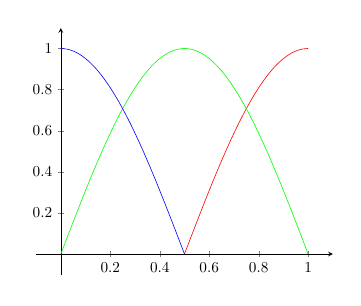
\begin{tikzpicture}[scale=0.55]
			\begin{axis}[
				trig format plots=rad,
				axis lines = middle,
				enlargelimits,
				clip=false
				]
				\addplot[domain=0.5:1,samples=200,red] {sin(pi*x - pi/2.0)};
				\addplot[domain=0:1,samples=200,green] {sin(x*pi)};
				\addplot[domain=0:0.5,samples=200,blue] {sin(pi*x + pi/2.0)};
				
			\end{axis}
		\end{tikzpicture}
	\caption{\textit{Mapping function from pixel difference to RGB components}}
	\label{fig:heat_sine}
	\end{figure}
	The CPU implementation is the following:
	\begin{lstlisting}[style=CStyle]
struct HeatElemt {
	int r;
	int g;
	int b;
};

HeatElemt getHeatPixel(int diff){
	struct HeatElemt h;
	float diff1 = diff/(255.0*2.0);
	
	// Map the difference into the three color components
	h.r = min(max(sin(M_PI*diff1 - M_PI/2.0)*255.0, 0.0),255.0);
	h.g = min(max(sin(M_PI*diff1)*255.0, 0.0),255.0);
	h.b = min(max(sin(M_PI*diff1 + M_PI/2.0)*255.0, 0.0),255.0);
}

while (1) {
	cap >> image2;
	for (int y = 0; y < H; y++){
		for (int x = 0; x < W; x++){
			Vec3b & intensity = image1.at<Vec3b>(y, x);
			Vec3b a = image1.at<Vec3b>(y, x);
			Vec3b b = image2.at<Vec3b>(y, x);
			
			// Compute the absolute difference
			HeatElemt elem = getHeatPixel(abs(a.val[0] - b.val[0]) + 
			abs(a.val[1] - b.val[1]) + abs(a.val[2] - b.val[2]));
			
			intensity.val[0] = elem.b;
			intensity.val[1] = elem.g;
			intensity.val[2] = elem.r;
		}
	}
	image1 = image2.clone();
}\end{lstlisting}
	In this CPU implementation, a loop is performed over each pixel of the two frames and the absolute difference computed. Another function, called \texttt{getHeatPixel} is used to convert that value to the heat map RGB color space. At this point, the original image is overwritten with the heatmap colors.

	
	\subsection{CUDA implementation}
	
	The idea is to rewrite what described in the previous section into a CUDA code. The GPU allows to run in parallel multiple instance of the same kernel, so that the execution can be done in parallel in order to speed up the computation.
	
	From the perspective of the interaction, the GPU acts like an accelerator of the CPU, that ask it to execute the kernel by resorting to the following phases:
	\begin{enumerate}
		\itemsep0sp
		\item Copy the frames from the Host to the Device memory
		\item Execute the kernel and wait its completion
		\item Retrieve the result from the Device to the Host memory
	\end{enumerate}
	
	This is exactly what the next section will explain. The kernel call allows to configure how many thread per kernel will be executed; obviously, depending on that number, the accessed locations must be defined accordingly. In fact, by defining $K$ the number of thread lunched, each thread will work on a specific portion of the entire image:
	\[
		\text{Thread portion dimension} = \frac{W \cdot H \cdot 3}{K}
	\]
	Where $W$ and $H$ are the width and height of the image. The multiplication by 3 depends on the fact that each pixels is defined by three \texttt{uint8\_t} datatype that each one of them defines a specific color. \newline\newline
	Furthermore, from the memory allocation perspective of the GPU, the memory for the two frames and the heat map must be allocated. This is done only once at the startup of the program, thanks to the CUDA API.	

\begin{lstlisting}[style=CStyle]
// Pointer definition
uint8_t *d_current, *d_previous;
uint8_t *d_heat_pixels;	

// Memory space reservion on GPU	
cudaMalloc((void **)&d_current, W*H*C * sizeof *d_current);
cudaMalloc((void **)&d_previous, W*H*C * sizeof *d_previous);
cudaMalloc((void **)&d_heat_pixels, W*H*C * sizeof *d_heat_pixels);\end{lstlisting}

	Unfortunately, this type of the problem doesn't need any shared or constant memory because each location in the image (all three colors of all pixels) are accessed only once and using a shared memory would have only reduced the performance due to the overhead of the useless copy. Moreover, there are no data that are constant.
	
	CUDA allows to get the information about the maximum number of thread by using the \texttt{cudaGetDeviceProperties} command and, by referring to the equation defined before, $K$ can be set to that value. In fact, the kernel is launched with the following configuration:
	\begin{itemize}
		\itemsep0sp
		\item \textit{Grid dimensions}:  1, 0, 0
		\item \textit{Block dimensions}: $K$, 0, 0
	\end{itemize}
	Having the maximum number of threads in the \texttt{threads} variable, it's possible to call the kernel in the following way:
	\begin{lstlisting}[style=CStyle]
// Kernel per block computation
cudaGetDeviceProperties(&prop, 0);
int threads = prop.maxThreadsPerBlock;
int maxSection = (W*H*C)/threads;\end{lstlisting}
	
	An extensive analysis of the correct number of threads has been done at Section \ref{sec:thread_n}.

	\subsubsection{CUDA Naif implementation}
	The first implementation of the algorithm in CUDA is based on a 1:1 transposition of what done in the CPU, in the GPU. Always using OpenCV, two next frames are fetched, send to the kernel and the heat map computed.
	
	\begin{lstlisting}[style=CStyle]
// Copy from Host to Device
cudaMemcpy(d_prev, image1,  W*H*C * sizeof *image1, cudaMemcpyHostToDevice);
cudaMemcpy(d_curr, image2,  W*H*C * sizeof *image2, cudaMemcpyHostToDevice);

kernel<<<1, threads>>>(d_curr, d_prev, maxSection, d_out);

// Copy heat map from Device to Host
cudaMemcpy(heatmap, d_out, W*H*C * sizeof *heatmap, cudaMemcpyDeviceToHost);\end{lstlisting}

	This naif implementation implies two memory transfers (HostToDevice) for the previous and current frames and one DeviceToHost for the generated heat map.
	
	
	In order to speed up the data management, instead of copying into a support array of \texttt{uint8\_t} the entire two frames (previous and current), both frames are directly copied into the device buffers with the \texttt{cudaMemcpy} procedure.\newline\newline
	Form the kernel perspective, there is a non-negligible complication with the respect to the CPU implementation. The CPU code is based on a single thread that iterates over the entire image in a sequential way, accessing one location after the other. For the GPU this is not the case, since now, each thread will work in parallel on a portion of the image that is long \texttt{maxSect}.
	
	Due to this, each kernel must know exactly from which pixel start to retrieve the data and where to store the results. This is only a matter of index management; let's suppose to have frame with dimension 1920*1080*3. So, by using 1024 threads per block, each thread will work on:
	\[
		maxSect = \frac{1920*1080*3}{1024} = 6075
	\]
	This means that the first thread must work from 0 to 6074, the second one from 6075 to 12149 and so on. This can be simply achieved by giving an univocal index identifier to each kernel, that cam be generated as:\newline\newline
	\texttt{int x = threadIdx.x + blockDim.x * blockIdx.x;}\newline\newline
	The GPU implementation of the first CUDA kernel is the following:
	\begin{lstlisting}[style=CStyle]
__global__ void kernel(uint8_t *current, uint8_t *previous,
					int maxSect, uint8_t* d_heat_pixels) {
	
	// Index relative to the block					
	int x = threadIdx.x + blockDim.x * blockIdx.x;
	
	// Start of the sector for this thread
	int start = x * maxSect;
	int max = start + maxSect;
	for (int i = start; i < max; i=i+C) {
		
		// Compute the pixel difference
		int pixelDiff = fabsf(current[i] - previous[i]) + fabsf(current[i+1]
				- previous[i+1]) + fabsf(current[i+2] - previous[i+2]); 
		float diff1 = pixelDiff/(255*2.0);
		
		// Map different into the three color component
		int r = fminf(fmaxf(__sinf(M_PI*diff1 - M_PI/2.0)*255.0, 0.0),255.0);
		int g = fminf(fmaxf(__sinf(M_PI*diff1)*255.0, 0.0),255.0);
		int b = fminf(fmaxf(__sinf(M_PI*diff1 + M_PI/2.0)*255.0, 0.0),255.0);
		d_heat_pixels[i] = b;
		d_heat_pixels[i+1] = g;
		d_heat_pixels[i+2] = r;
	}
} \end{lstlisting}
	
	After having run the \texttt{nvprof}, the main contributions to the execution time from the profiler are:
	\begin{figure}[H]
		\centering
			\begin{center}
			\begin{tabular}{ |c|c|c|c| } 
				\hline
				\textbf{Type} & \textbf{Time} (\%) & \textbf{Avg} & \textbf{Name} \\ 
				\hline
				GPU activities & 86.14 & 49.958 & kernel \\ 
				& 9.38 & 2.5577ms & [CUDA memcpy HtoD] \\ 
				& 4.48 & 2.4427ms & [CUDA memcpy DtoH] \\ 
				\hline
				API calls & 93.88 & 18.820ms & cudaMemcpy \\ 
				& 5.88 & 181.61ms & cudaMalloc \\ 
				\hline
			\end{tabular}
		\end{center}
		\label{fig:table_v1}
		\caption{\textit{Profiling result v1.cu}}
	\end{figure}
	In fact, the cumulative time needed to copy all two frames into the device, execute the kernel and copy back the image in order to display it, takes approximately 57ms. From the GPU perspective, the average time to execute one single kernel is 49.958ms.
	
		
	Even a very simple naif CUDA implementation can achieve a large performance improvement with the respect to the CPU. This is thanks to the \href{https://docs.nvidia.com/cuda/cuda-math-api/group__CUDA__MATH__INTRINSIC__SINGLE.html}{Single Precision Intrinsics} functions of CUDA. More precisely, the sine is computed by using the \texttt{\_\_sinf}, that allows to calculate the fast approximate sine of the input argument.
	
	\begin{figure}[H]
		\centering
		\begin{center}
			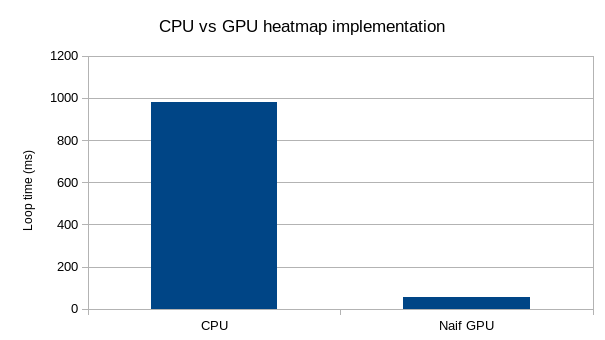
\includegraphics[width=0.35\linewidth]{images/heatmap/gpu_naif}
		\end{center}
	\label{fig:cpu_vs_gpu}
	\caption{\textit{Loop time CPU vs GPU}}
	\end{figure}
	
	\subsubsection{CUDA switching frames}
	
	The first idea to reduce the time used for copying the frames from the Host to the Device. Instead of copying each time both the two frame, one of the two can be reused by only switching the two points, so that the one that previously was the current will became the previous; at this point, only the new frame must be copied into the device memory. This means that approximately the \textit{CUDA memcpy HtoD} should be half of the previous time. This led to a \texttt{v2.cu} implementation, that exploit this pointer switching to reduce the memory transfer. The below code portion shows only the pointer switching in the loop used to fetch the frames.
		\begin{lstlisting}[style=CStyle]
while(1){
	// New frame fetch
	cap >> image2;
	
	// Pointer switching
	uint8_t* tmp = d_curr;
	d_curr = d_prev;
	d_prev = tmp;
	
	// Kernel call
	cudaMemcpy(d_curr, image2,  W*H*C * sizeof *image2, cudaMemcpyHostToDevice);
	kernel<<<1, threads>>>(d_curr, d_prev, (W*H*C)/threads, d_out);
	cudaMemcpy(heatmap, d_out, W*H*C * sizeof *heatmap, cudaMemcpyDeviceToHost);
	
	image1 = image2.clone();
}\end{lstlisting}
	
	\begin{figure}[H]
		\centering
		\begin{center}
			\begin{tabular}{ |c|c|c|c| } 
				\hline
				\textbf{Type} & \textbf{Time} (\%) & \textbf{Avg} & \textbf{Name} \\ 
				\hline
				GPU activities & 90.54 & 46.023 & kernel \\ 
				& 4.85 & 2.4400ms & [CUDA memcpy HtoD] \\ 
				& 4.61 & 2.3453ms & [CUDA memcpy DtoH] \\ 
				\hline
				API calls & 89.88 & 26.026ms & cudaMemcpy \\ 
				& 9.90 & 192.15ms & cudaMalloc \\ 
				\hline
			\end{tabular}
		\end{center}
		\label{fig:table_v2}
		\caption{\textit{Profiling result v2.cu}}
	\end{figure}
	The average kernel execution time is in ms, and it is not a figure of interest, since it is more or less equal to the previous version. What is important is that now, the percentage of time used for the kernel is increase, due to the reduced \textit{CUDA memcpy HtoD} (from  9.38\% to 4.85\%). This means that the GPU will analyze more frame in the same time frame. As we would expect, now the time needed to copy a frame from the memory to the device, execute the kernel and then retrieve the heat map takes about 50ms (12\% faster).
	
	\subsubsection{CUDA Global memory access granularity}
	The problem with the generation of the heat map is that, the computation of the color must be done every time for all the pixels in order to compute the complete image.\newline\newline
	Since each thread must perform 6075 iterations and need to write on the Global memory the same amount of times.
	In order to reduce the number of accesses to the Global memory, the idea was to access at the \texttt{int} level instead of the \texttt{byte} level. This means that frame information are still copied from host to device as arrays of \textit{bytes} but they are accesses at the int level. So, if the current and the previous frames are passed as \texttt{uint8\_t *current, uint8\_t *previous}, the access is aligned at the 4 bytes. 
	Another problem arises: the threads now access the memory with a granularity of 4 byte, but since the pixel difference needs needs only the first three bytes (RGB), in order to optimize and avoid to read twice from the memory, colors are updated only once every 3 bytes. So, when the position of the color in the image is the first, the colors of the heat map are set in the current and next two bytes of the output array, accordingly to the computed difference.
	\begin{lstlisting}[style=CStyle]
__global__ void kernel(uint8_t *current, uint8_t *previous,
					int maxSect, uint8_t* d_heat_pixels) {
	int x = threadIdx.x + blockDim.x * blockIdx.x;
	int start = x * maxSect;
	int max = start + maxSect;
	int cc, pc;
	for (int i = start; i < max; i++) {
		
		// Access one 4 byte at a time
		cc = ((int *)current)[i];
		pc = ((int *)previous)[i];
		int pixelDiff = 0;
		for (int j = 0; j < 4; j++) {
			
			// Conversion from difference to heat map only every 3 bytes
			if((i*4+j) % 3 == 0){
				int pixelDiff = fabsf(((uint8_t *)&cc)[j] - ((uint8_t *)&pc)[j]) +
				fabsf(((uint8_t *)&cc)[j+1] - ((uint8_t *)&pc)[j+1]) +
				fabsf(((uint8_t *)&cc)[j+2] - ((uint8_t *)&pc)[j+2]);
				float diff1 = pixelDiff/(255*2.0);
				int r = fminf(fmaxf(sinf(M_PI*diff1 - M_PI/2.0)*255.0, 0.0),255.0);
				int g = fminf(fmaxf(sinf(M_PI*diff1)*255.0, 0.0),255.0);
				int b = fminf(fmaxf(sinf(M_PI*diff1 + M_PI/2.0)*255.0, 0.0),255.0);
				d_heat_pixels[i*4+j] = b;
				d_heat_pixels[i*4+j+1] = g;
				d_heat_pixels[i*4+j+2] = r;
				
				// Reset the pixel difference
				pixelDiff = 0;
			}
		}
	}
}\end{lstlisting}
	Since now each threads works on 4 bytes at a iteration, the dimension of the data section that each block must work on is reduced by $1/4$, as in the following way:
		\begin{lstlisting}[style=CStyle]
cudaGetDeviceProperties(&prop, 0);
int threads = prop.maxThreadsPerBlock;

cudaMemcpy(d_curr, image2,  W*H*C * sizeof *image2, cudaMemcpyHostToDevice);

// Kernel call /4
kernel<<<1, threads>>>(d_curr, d_prev, ((W*H*C)/threads)/4, d_out);
cudaMemcpy(heatmap, d_out, W*H*C * sizeof *heatmap, cudaMemcpyDeviceToHost);\end{lstlisting}

	This led to another version, available at \texttt{v3.cu} allows to obtain the following results:
	\begin{figure}[H]
		\centering
		\begin{center}
			\begin{tabular}{ |c|c|c|c| } 
				\hline
				\textbf{Type} & \textbf{Time} (\%) & \textbf{Avg} & \textbf{Name} \\ 
				\hline
				GPU activities & 84.08 & 25.457ms & kernel \\ 
				& 8.14 & 2.4405ms & [CUDA memcpy HtoD] \\ 
				& 7.78 & 2.3549ms & [CUDA memcpy DtoH] \\ 
				\hline
				API calls & 85.73 & 15.810ms & cudaMemcpy \\ 
				& 13.93 & 172.12ms & cudaMalloc \\ 
				\hline
			\end{tabular}
		\end{center}
		\label{fig:table_v3}
		\caption{\textit{Profiling result v3.cu}}
	\end{figure}
	
	This version allows to copy the next frame from memory to device, execute the kernel and retrieve the result in about 30ms (about 40\% of performance increase from \texttt{v2.cu}). This is highlighted in the table by the average time needed to execute the kernel itself, we went from 46.023ms to 25.457ms, thanks to the reduce access time to the memory.
	
	\subsection{Evaluation of the number of threads}
	\label{sec:thread_n}
	For a first implementation, the number of thread has been set to the maximum allowable from the architecture, that is given by the \texttt{cudaGetDeviceProperties} CUDA function in order to make the program independent form the device used. For example, for the Jetson Nano, the maximum number of threads are 1024.\newline\newline
	In order to understand how the number of threads impacts on the heat map generation, a bash script has been build in order to dynamically change the $K$ parameter via compiler directive. The number of threads must be a multiple of 4, so that the array of the pixels can be divided into portion in such a way that a pixel is not split between two kernel.
	
	This is the bash code used to extract the \textit{nvprof} information:
	\begin{lstlisting}[language=bash]
#!/bin/bash
for i in {1..256}
do
	k=$(( 4*i ))
	
	# Profiler call
	avg=`sudo /usr/local/cuda/bin/nvprof ./heatMap $k 2>&1`
	
	# Data extraction
	kern=`echo "$avg" | grep kernel | awk '{print $6}'`
	kernt=`echo "$avg" | grep kernel | awk '{print $4}'`
	hd1=`echo "$avg" | grep "CUDA memcpy HtoD" | awk '{print $4}'`
	hd2=`echo "$avg" | grep "CUDA memcpy HtoD" | awk '{print $2}'`
	dh1=`echo "$avg" | grep "CUDA memcpy DtoH" | awk '{print $4}'`
	dh2=`echo "$avg" | grep "CUDA memcpy DtoH" | awk '{print $2}'`
	echo "$k $all $kern $kernt $hd1 $hd2 $dh1 $dh2" >> times.txt
done\end{lstlisting}
	In this way, the output of the profiler and the time needed to copy the frame, generate the heat map and retrieve the result is parsed and wrote into a file called \texttt{times.txt}. Thanks to another script, the most useful data are plot, as below:
	
	\begin{figure}[H]
		\centering
		\begin{subfigure}{.45\textwidth}
			\centering
			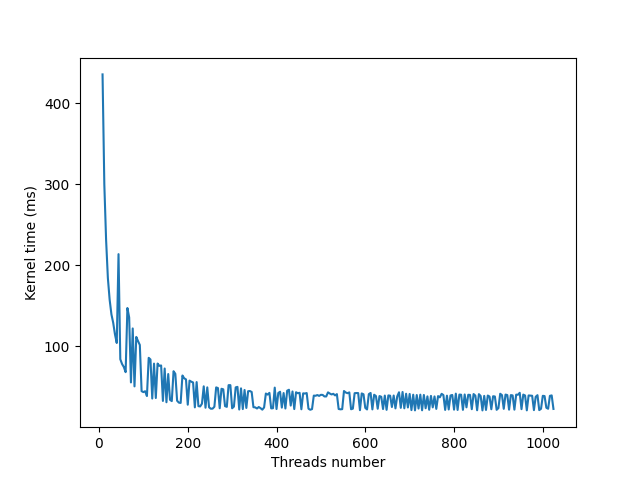
\includegraphics[width=.8\linewidth]{images/heatmap/plot_kernel_times.png}
			\caption{Time needed to perform an heatmap depending on the number of kernel set}
			\label{fig:sub1}
		\end{subfigure}%
		\hspace{5mm}
		\begin{subfigure}{.45\textwidth}
			\centering
			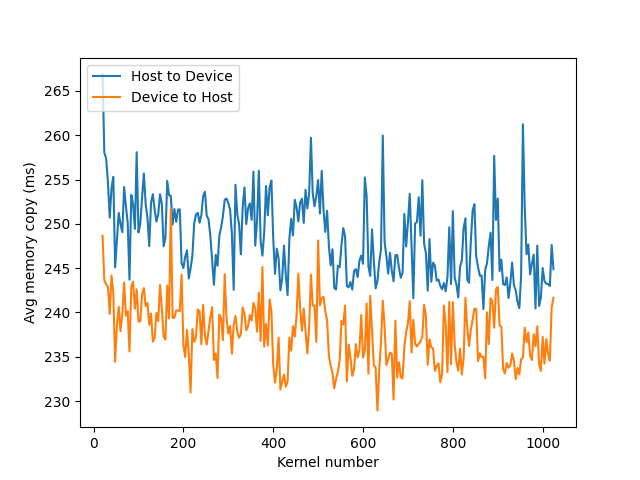
\includegraphics[width=.8\linewidth]{images/heatmap/hd.png}
			\caption{Time needed to copy from Host to Device (blue) and from Device to Host (orange)}
			\label{fig:sub2}
		\end{subfigure}
	\end{figure}
	This is not the behaviour that we would have expected, beside the time needed to copy is more or less constant, by increasing the number of threads for that kernel we would expect that the time needed for the heat map computation would be lower. This is probably due to the fact that the \textit{warp} has a fixed size of 32 threads and, even if by increasing the number of threads its execution time is lower, their management probably introduce too much overhead to obtain benefits.
	
	Beside this, the time needed to perform an heatmap vs the number of threads, shows a peculiar behaviour. After about $N > 280$ the times tend to oscillate between more or less 50ms and 27ms. Even if this seems not a big difference, in the filed of real-time image processing, it's a huge improvement. In order to avoid errors, the same script has been run multiple times and the results is always the same. Since the internal infrastructure is a black box, the hardware probably manage in different ways the threads with the respect to their number.\newline
	The best observed thread configuration for the Jetson Nano, seems to be 716.\newline\newline
	In fact, by running the same exact algorithm describe before but the number of threads is set to 718 (that is the best kernel accordingly to the plot above), the time needed to copy a frame, compute the heat map and then copy back the heat map matrix is about 27ms. This leads to a increasing of performance of 10\%, that in this domain is not negligible.
	
	The following table shows some meaningful data extracted from the profiler:
		\begin{figure}[H]
		\centering
		\begin{center}
			\begin{tabular}{ |c|c|c|c| } 
				\hline
				\textbf{Type} & \textbf{Time} (\%) & \textbf{Avg} & \textbf{Name} \\ 
				\hline
				GPU activities & 84.30 & 24.380ms & kernel \\ 
				& 8.04 & 2.4599ms & [CUDA memcpy HtoD] \\ 
				& 7.66 & 2.383ms & [CUDA memcpy DtoH] \\ 
				\hline
				API calls & 90.06 & 16.192ms & cudaMemcpy \\ 
				& 9.57 & 115.27ms & cudaMalloc \\ 
				\hline
			\end{tabular}
		\end{center}
		\label{fig:table_v4}
		\caption{\textit{Profiling result v3.cu}}
	\end{figure}

	\subsubsection{Heatmap Conclusions}

	By considering only the CUDA algorithm, the optimizations shows a decreasing fashion of the time needed to process the two frames and generate the heat map. The Loop average time, is the time needed to copy the image from the Host to the Device, summed to the heat map time computation and the time needed to copy it back. On the other hand, the plot on the right shows only the average kernel time. All data are in ms. 
	\begin{center}
		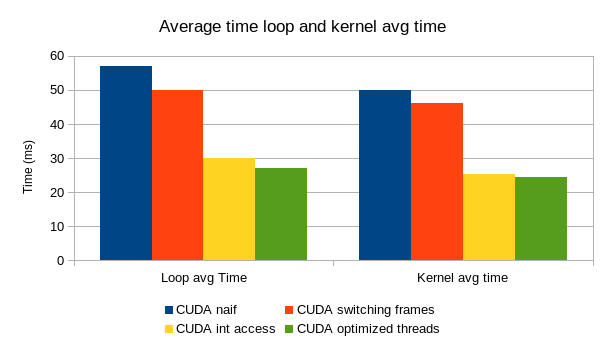
\includegraphics[width=0.65\linewidth]{images/heatmap/histo_results}
	\end{center}
	
	
	\section{Noise visualizer}
	\label{sec:noise_visualizer}
	As already explained in the first sections, the algorithm is based on sending only the difference of all pixels whose color components are above a certain threshold.
	
	In order to better visualize the noise in each frame taken from the webcam, all colors of all pixels that are above a certain threshold, are colored in red. The threshold is the same used by the kernel that computes all pixel differences. Obviously, the complexity of this computation is much easier than the previous one and the CPU allows to compute that kind of map in around 250ms.
	\begin{figure}[H]
		\centering
		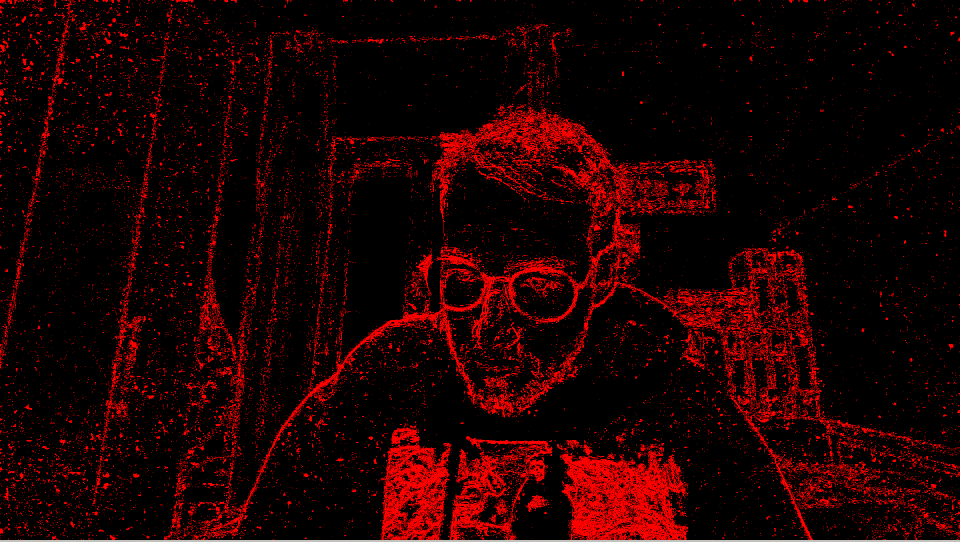
\includegraphics[width=0.4\linewidth]{images/heatmap/v0-red}
		\caption{\textit{All non normalized pixel difference are turned to red if above a certain threshold, in this case 20. Beside the figure in the center, all red pixels can be identified as noise.}}
		\label{fig:v0-red}
	\end{figure}
	The purpose of this new color mapping is completely different from the heatmap, since the latter one is used to understand the magnitude of the pixel difference while the second one (the black-red) is used to better visualize the noise pixels, by using a threshold.
	
	\textit{Why is this necessary?} This allows to have a visual evaluation of the noise filter, that is used to reduce smooth the noise in order to reduce the difference between two frames and reduce even more the bandwidth. The noise filter will be explained in the next section.\newline\newline
	First of all, we need to define what is the noise: by means of noise we are referring to all the random variations on the color information in an image, that is visible as grain in film and pixel level. The level of the noise mainly depends:
	\begin{itemize}
		\itemsep0sp
		\item Length of the exposure
		\item Sensitivity of the optical camera
		\item Brightness of the environment
		\item Temperature
	\end{itemize}
	In most of the cases, the webcam used at home is a cheap one that has an extremely small pixels in the camera sensor. There are mainly three types of noises: fixed pattern noise, random noise and banding noise. The common noise in our webcam is the one shown below. As you can see, the dark and less brightness parts of the image are characterized by some particles that shows different color from the whole context. 
	\begin{figure}[H]
		\centering
		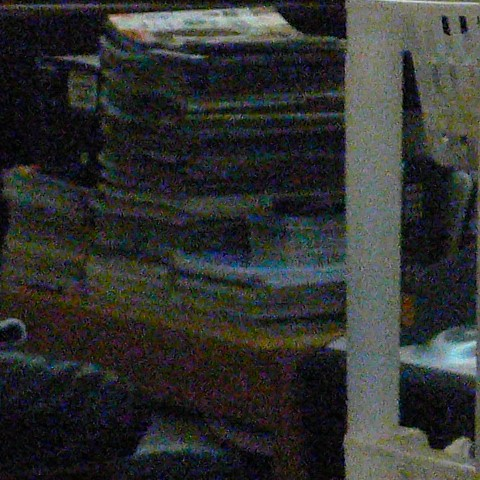
\includegraphics[width=0.25\linewidth]{images/heatmap/noise}
		\caption{\textit{Example of noise}}
		\label{fig:noise}
	\end{figure}
	From our perspective this is a very bad behaviour due to the fact that the noise is random, and can change the value of the pixel at each frame. This leads to an high amount of pixel changed, even if the image is always the same. For this reason, \textit{noise image filtering} is performed over the frame, before being analyzed by the CUDA kernel that computes the pixel differences.\newline\newline

	The internal logic of a webcam allows to trim some parameters of the video capture directly by OpenCV. This is not a software level manipulation of the frame, but the internal control unit of the webcam, while sampling the frame, performs different behaviour depending on the selected configuration. 
	
	For this reason, the original image has been enhanced with a control panel, so that the user can change the brightness, the contrast, the saturation and the gain of the image. The Figure \ref{fig:controls}, shows the panel that is shown to the user. Even if it can be used to reduce the noise, by for example reducing the contrast, it allows the user to increase the quality of the send image.
	\begin{figure}[H]
		\centering
		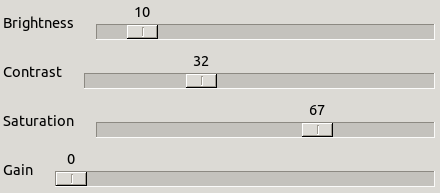
\includegraphics[width=0.33\linewidth]{images/heatmap/controls}
		\caption{\textit{Image Control panel}}
		\label{fig:controls}
	\end{figure}
	
	\subsubsection{Naif CPU implementation}
	The \textit{naif} CPU implementation starts from the same program base used for the heat map. The entire image, pixel by pixel, is analyzed and if one of the color component is above the same threshold set for the pixel difference, that pixel is colored in red otherwise in black.
	
	The code below is the C implementation of what explained before, where \texttt{LR\_THRESHOLDS} is set to 20.
\begin{lstlisting}[style=CStyle]
for (int y = 0; y < H; y++){
	for (int x = 0; x < W; x++){
		Vec3b & intensity = image1.at<Vec3b>(y, x);
		Vec3b a = image1.at<Vec3b>(y, x);
		Vec3b b = image2.at<Vec3b>(y, x);
		
		if(abs(a.val[0] - b.val[0]) > LR_THRESHOLDS ||
					abs(a.val[1] - b.val[1]) > LR_THRESHOLDS ||
					abs(a.val[2] - b.val[2]) > LR_THRESHOLDS)
		{
			intensity.val[0] = 0;
			intensity.val[1] = 0;
			intensity.val[2] = 255;
		} else {
			intensity.val[0] = 0;
			intensity.val[1] = 0;
			intensity.val[2] = 0;
		}
	}
}\end{lstlisting}
	The resulting image is the one at Figure \ref{fig:v0-red}. From the time perspective, as said before, being the operations for the noise visualizer less complex, the CPU is able to generate the image in around 250ms.
	
	\subsubsection{CUDA implementation}
	The same considerations and optimization steps done for the heat map can be done also for the generation of the frames that allows the user to better visualize the noise in the frames. So, starting from an already optimized memory management, the resulting kernel call is based as always on first copy the frame into the Device Global memory, call the kernel and then retrieve the image, as in the code below:
\begin{lstlisting}[style=CStyle]
	cudaGetDeviceProperties(&prop, 0);
	int threads = prop.maxThreadsPerBlock;
	
	cudaMemcpy(d_curr, image2,  W*H*C * sizeof *image2, cudaMemcpyHostToDevice);
	
	// Kernel call /4
	kernel_red<<<1, threads>>>(d_curr, d_prev, ((W*H*C)/threads/
																(sizeof(chunk_t)), d_out);
	cudaMemcpy(heatmap, d_out, W*H*C * sizeof *heatmap, cudaMemcpyDeviceToHost);\end{lstlisting}
	
	In this case, the optimization described in the pixel difference generation, regarding the \textit{vectorized access} to memory is also applied here, where a new type called \texttt{chunk\_t} is defined. In this way more byte can be read with a single memory access.
	
	\begin{lstlisting}[style=CStyle]
typedef int4 chunk_t;
	
__global__ void kernel_red(uint8_t *current, uint8_t *previous,
					int maxSect, uint8_t* d_heat_pixels) {
	int x = threadIdx.x + blockDim.x * blockIdx.x;
	int start = x * maxSect;
	int max = start + maxSect;
	chunk_t cc, pc;
	
	uint8_t redColor = 0;
	for (int i = start; i < max; i++) {
		cc = ((chunk_t *)current)[i];
		pc = ((chunk_t *)previous)[i];
		for (int j = 0; j < sizeof cc; j++) {
			int8_t df = ((uint8_t *)&cc)[j] - ((uint8_t *)&pc)[j];
			
			if (df < -LR_THRESHOLDS || df > LR_THRESHOLDS) {
				redColor = 255;
			}
			
			// Access to the global memory
			if((i*(sizeof cc)+j) % 3 == 2){
				d_heat_pixels[i*(sizeof cc)+j] = redColor;
				redColor = 0;
			}  else {
				d_heat_pixels[i*(sizeof cc)+j] = 0;
			}
		}
	}
}	\end{lstlisting}
	By iteration on all the color components of all the pixels in the frame, the difference with the previous frame is checked. If it is above the threshold, the value of the red color for that pixel is set to 255. 
	
	Being the red component the third in a pixel, it is set accordingly to the \texttt{redColor} variable only if the \texttt{i*(sizeof cc) + j \% 3 == 2} (the red color).\newline\newline
	This implementation allows to copy the frame from Host to Device, compute the noise visualization and retrieve back the image from Device to Host memory in around 26ms.
	
	The following table shows some meaningful data extracted from the profiler:
	\begin{figure}[H]
		\centering
		\begin{center}
			\begin{tabular}{ |c|c|c|c|c|c| } 
				\hline
				\textbf{Type} & \textbf{Time} (\%) & \textbf{Avg} & \textbf{Min} & \textbf{Max} & \textbf{Name} \\ 
				\hline
				GPU activities & 81.38 & 21.759 & 19.489 & 32.94 & kernel\_red \\ 
				& 9.59 & 2.5469 & 2.2134 & 6.8552 & [CUDA memcpy HtoD] \\ 
				& 9.03 & 2.4141 & 2.1828 & 3.5408 & [CUDA memcpy DtoH] \\ 
				\hline
				API calls & 87.41 & 13.992 &  2.7579 & 156.01 & cudaMemcpy \\ 
				& 12.13 & 194.86  & 3.8501 & 576.73 & cudaMalloc \\ 
				\hline
			\end{tabular}
		\end{center}
		\label{fig:table_v1_red}
		\caption{\textit{Profiling result v1.cu for noise visualizer}}
	\end{figure}
	As you can see, the average time needed to compute the kernel is less with the respect to the heat map. This is due to the simplicity of the function that only need to check the difference against a threshold. As you can see, the GPU acceleration has a huge impact over the computation.
	\begin{center}
		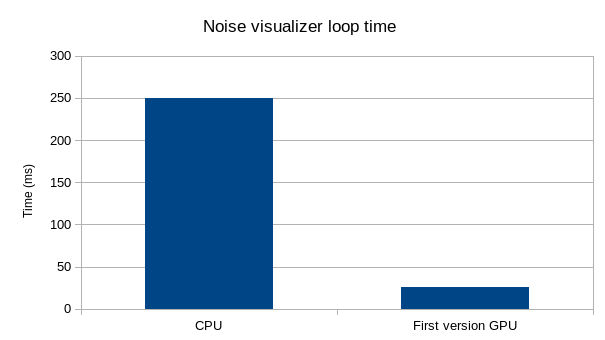
\includegraphics[width=0.35\linewidth]{images/heatmap/noise1}
	\end{center}
	
	
	\subsubsection{CUDA reduction of global memory accesses}
	The fact that the only pixels that changes is the red one, the previous CUDA kernel can be optimized even more in order to reduce the number of access to the global memory. In fact, if we set assume that at the beginning all pixels in the \texttt{d\_heat\_map} array are all completely black, the algorithm can reduce the memory access of on third since it will work only on a the red color component. As before, if the difference is above a threshold, the red pixel is turned to red, or to black otherwise.

	The resulting kernel is the following:
	
\begin{lstlisting}[style=CStyle]
	typedef int4 chunk_t;
	
	__global__ void kernel_red(uint8_t *current, uint8_t *previous,
	int maxSect, uint8_t* d_heat_pixels) {
		int x = threadIdx.x + blockDim.x * blockIdx.x;
		int start = x * maxSect;
		int max = start + maxSect;
		chunk_t cc, pc;
		
		uint8_t redColor = 0;
		for (int i = start; i < max; i++) {
			cc = ((chunk_t *)current)[i];
			pc = ((chunk_t *)previous)[i];
			for (int j = 0; j < sizeof cc; j++) {
				int8_t df = ((uint8_t *)&cc)[j] - ((uint8_t *)&pc)[j];
				
				if (df < -LR_THRESHOLDS || df > LR_THRESHOLDS) {
					redColor = 255;
				}
				
				// Access to the global memory
				if((i*(sizeof cc)+j) % 3 == 2){
					d_heat_pixels[i*(sizeof cc)+j] = redColor;
					redColor = 0;
			}
		}
	}
}	\end{lstlisting}
	As you can notice, the only difference is that the else condition is the last if statement has been removed. This means that the green and blue component are not modified, thus the global memory is left as is for these two bytes.
	
	This allowed to increase the performance of the kernel even more; as you can see from the table below the kernel now lasts in average 16.684ms, that is a 23\% faster. The entire loop is done in about 22ms. \newline\newline
	Moreover, the test must be performed in the same conditions because, depending on the video captured, it can show different number of changed pixels with the value of the difference above or below the threshold. For this reason, the \textit{nvprof} has been run while the webcam was covered with a black tape. Due to the fashion of the algorithm, also the minimum and maximum values have been included in the table below.

	\begin{figure}[H]
		\centering
		\begin{center}
			\begin{tabular}{ |c|c|c|c|c|c| } 
				\hline
				\textbf{Type} & \textbf{Time} (\%) & \textbf{Avg} & \textbf{Min} & \textbf{Max} & \textbf{Name} \\ 
				\hline
				GPU activities & 75.63 & 16.684 & 16.372 & 35.942 & kernel\_red \\ 
							   & 12.37 & 2.6294 & 2.2265 & 6.3841 & [CUDA memcpy HtoD] \\ 
							   & 12.00 & 2.6294 &  2.2265 & 6.3841 & [CUDA memcpy DtoH] \\ 
				\hline
				API calls & 86.00 &  11.610 & 2.6999 & 41.414 & cudaMemcpy \\ 
						  & 13.56 & 183.71 & 3.7352 & 543.50 & cudaMalloc \\ 
				\hline
			\end{tabular}
		\end{center}
		\label{fig:table_v2_red}
		\caption{\textit{Profiling result v2.cu for noise visualizer}}
	\end{figure}

	The code of this and the previous implementation has been disassembled using the NVIDIA tools \textit{cuobjdump} and \textit{nvdisasm}; the last one is also needed to get information about the control flow. In order to avoid that the \textit{nvcc} compiler to avoid, with very limited exceptions, dead-code eliminations and register-spilling optimizations. For this reason the code has been compiled with the \texttt{-O0} flag.

	The generation of the assembly is:
	\begin{lstlisting}[language=bash]
cuobjdump ./a.out -xelf all
nvdisasm v1.sm_30.cubin\end{lstlisting}
	
	By looking carefully at the assembly code of the first implementation, it's possible to understand the correlation between the assembly code and the instructions. As we would have expected, in the code of the first implementation are present two \texttt{ST.E.U8} instructions, used to perform the if and else case.
	
	The following is an extract of the assembly that manage the if statement on the first CUDA implementation.
	\begin{figure}[H]
		\begin{lstlisting}[style=CStyle]
	// Perform comparison
	/*0ab0*/ ISETP.EQ.X.AND P0, PT, R5, RZ, PT;
	/*0ab8*/ PSETP.AND.AND P0, PT, !P0, PT, PT;
	/*0ac8*/ SSY `(.L_16);
	
	// Go to if
	/*0ad0*/ @P0 BRA `(.L_17);
	
	// Go to else
	/*0ad8*/ BRA `(.L_18);



// IF
.L_17
	...
	/*0e10*/ ST.E.U8 [R4], R0;
	/*0e28*/ NOP.S (*"TARGET= .L_16 "*);

// ELSE
.L_18:
	...
	/*0c50*/ ST.E.U8 [R4], R0;
	/*0c88*/ NOP.S (*"TARGET= .L_16 "*);


// Management of the loop control flow	
.L_16
	...\end{lstlisting}
	\caption{Assembly extract of the first CUDA implementation of the noise visualizer}
	\end{figure}

	So, label \texttt{.L\_17} and \texttt{.L\_18} are used to identify the branch that is used to write 0 or 255, accordingly to the fact that it is or not the red component and only if above the threshold.\newline\newline
	On the other hand, the assembly of the second implementation shows only one instance of the store byte instruction, as we would have expected:
	\begin{figure}[H]
	\begin{lstlisting}[style=CStyle]
	// Perform comparison
	/*0aa8*/ IADD32I RZ.CC, R4, -0x2;
	/*0ab0*/ ISETP.EQ.X.AND P0, PT, R5, RZ, PT;
	/*0ab8*/ PSETP.AND.AND P0, PT, !P0, PT, PT;
	/*0ac8*/ PRMT R0, R29, 0x7610, R0;
	/*0ad0*/ PSETP.AND.AND P0, PT, P0, PT, PT;
	/*0ad8*/ PRMT R0, R0, 0x7610, R0;
	/*0ae0*/ SSY `(.L_16);
	/*0ae8*/ @P0 NOP.S (*"TARGET= .L_16 "*);
	/*0af0*/ BRA `(.L_17);


// IF
.L_17
	...
	/*0e10*/ ST.E.U8 [R4], R0;
	/*0e28*/ NOP.S (*"TARGET= .L_16 "*);


// Management of the loop control flow	
.L_16
	...\end{lstlisting}
	\caption{Assembly extract of the second CUDA implementation of the noise visualizer}
	\end{figure}
	

	
	\subsubsection{Fastest implementation}
	The fact that the we can have a frame that changes completely with the respect to the previous one, implies that not only the black pixels must be turned in red if above a certain threshold, but also the red ones that are below must be changed to black. This means that we if we have an image $1920*1080*3$ we can't go below $1920*1080$ access to Global Memory. 
	
	A second approach resort to not use the output \texttt{d\_heat\_pixels} as output array but instead write directly over the \textit{previous} frame. In this way, the red pixel will be placed over the frame itself; this is a completely different representation but, if we can modify the original frame (that will be discharged at the end of the loop), this solution is feasible. The result is visible at Figure \ref{fig:red_frame}.
	
	\begin{figure}[H]
		\centering
		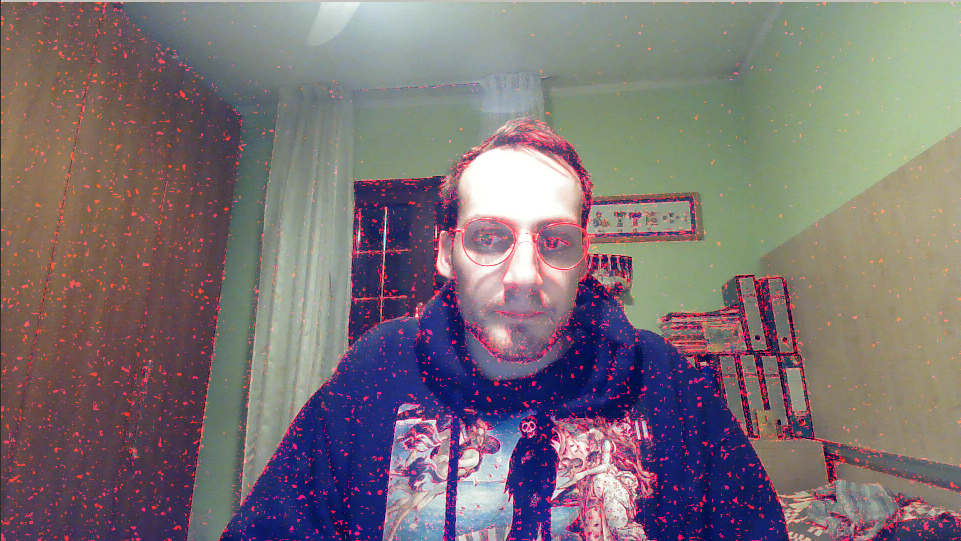
\includegraphics[width=0.45\linewidth]{images/heatmap/gpu_red_2}
		\caption{\textit{Red pixels over the frame}}
		\label{fig:red_frame}
	\end{figure}
	
	This has be done to overcome the need of setting a pixel to black when the difference between the pixels is below the threshold. With this approach, the number of write to the Global Memory should corresponds to the number of pixels whose difference is above the threshold. Hypothetically, two identical frames should not need any write access to the Global Memory.
	
	The kernel has been modified in the following way, so that the red color is set only if at least one color component of that pixel is above the threshold:
\begin{lstlisting}[style=CStyle]
typedef int4 chunk_t;

__global__ void kernel_red(uint8_t *current, uint8_t *previous,
int maxSect) {
	int x = threadIdx.x + blockDim.x * blockIdx.x;
	int start = x * maxSect;
	int max = start + maxSect;
	chunk_t cc, pc;
	
	bool toUpdate = false;
	for (int i = start; i < max; i++) {
		
		cc = ((chunk_t *)current)[i];
		pc = ((chunk_t *)previous)[i];
		for (int j = 0; j < sizeof cc; j++) {
			int8_t df = ((uint8_t *)&cc)[j] - ((uint8_t *)&pc)[j];
			
			if (df < -LR_THRESHOLDS || df > LR_THRESHOLDS) {
				toUpdate = true;
			}
			
			// Update only if needed
			if (toUpdate && (i*(sizeof cc)+j) % 3 == 2){
			previous[i*(sizeof cc)+j] = 255;
			toUpdate = false;
		}
	}
}	\end{lstlisting}

	Obviously, also the kernel call must be modified, so that instead of copying back data from the \texttt{d\_heat\_map} the data are retrieved from the previous frame, that has been overwrite during the kernel execution:
	
\begin{lstlisting}[style=CStyle]
cudaMemcpy(d_current, image2.data,  W*H*C * sizeof *image2.data,
												cudaMemcpyHostToDevice);
kernel<<<1, threads>>>(d_current, d_previous, (((W*H*C)/threads)/
												(sizeof(chunk_t))));

// Rewrite d_previous frame
cudaMemcpy(res.data, d_previous, W*H*C * sizeof *res.data,
											cudaMemcpyDeviceToHost);\end{lstlisting}	
										
										
	This implementation, in the same test condition that has been used also for the other two implementations of the noise visualizer, allows to perform the copy of the frame from Host to Device, compute the noise visualization and copy it from the Global memory of the Device to the Host in around 16.5ms.
	
	These are the results from \textit{nvprof}:
	\begin{figure}[H]
		\centering
		\begin{center}
			\begin{tabular}{ |c|c|c|c|c|c| } 
				\hline
				\textbf{Type} & \textbf{Time} (\%) & \textbf{Avg} & \textbf{Min} & \textbf{Max} & \textbf{Name} \\ 
				\hline
				GPU activities & 53.05 & 7.5647 &  4.9421 &  51.426 & kernel\_red \\ 
				& 23.69 & 3.3450 & 2.4960 & 6.6161 & [CUDA memcpy HtoD] \\ 
				& 23.26 & 3.3160 & 2.8359 & 4.2297 & [CUDA memcpy DtoH] \\ 
				\hline
				API calls & 81.86 &  7.7539 &  2.9697 &  57.082 & cudaMemcpy \\ 
				& 17.51 & 166.67 & 5.4298 & 327.91 & cudaMalloc \\ 
				\hline
			\end{tabular}
		\end{center}
		\label{fig:table_v3_red}
		\caption{\textit{Profiling result v3.cu for noise visualizer, overwriting the red pixels over the previous frame}}
	\end{figure}
	
	As you can see from the time for the kernel execution, there is a huge improvement from the black and red implementation of about 25\% more.
	
	\begin{figure}[H]
		\centering
		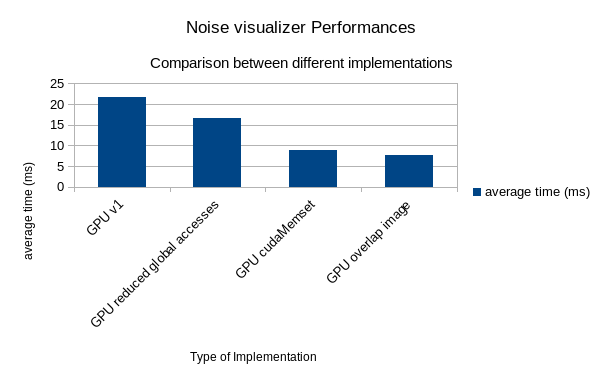
\includegraphics[width=0.35\linewidth]{images/heatmap/noise2}
		\caption{\textit{Comparison between GPU versions for noise visualizer}}
		\label{fig:noise2}
	\end{figure}

	\section{Noise filter}
	The sensor of an digital camera contains a certain number of pixel, used to acquire the image. The settings of a camera allows to adapt the sensor to the external conditions in order to always get the best shot). In a sunny day, a slow  shutter speed, a wide open aperture allows a large number of photons to hit completely the image sensor.
	
	On the other hand, in darker conditions, faster shutter speeds and a closer aperture do not allow enough photons to hit the sensor to generate a suitable voltage to overcome the noise present at the ground. This leads to a low Signal-To-Noise ratio that is directly converted into noise from the internal camera logic. In this case, a correct trim of the of ISO and the shutter aperture time allow to have an image with lower noise; but, in most of the cases, the cheap webcams do not have these advanced configurable feature but perform an auto-adapt procedure.\newline\newline
	This is where the \textit{noise filtering} take a major role for this project. Being the data sent based on the difference with the previous frame, each pixel that is mainly driven by the noise, has higher probability to flip drastically change its value. So, even if the pixel itself does not contains any information, its difference is still sent.
	
	\subsection{Convolution filters}
	Convolution filters are used to perform some perturbation over an image in order to obtain some enhancement. They are based on a \textit{kernel}, a convolution matrix, that is used to perform the convolution between the image and the kernel itself, in the following way:
	
	\begin{align*}
		g(x,y) = \sum_{u = \frac{-k}{2}}^{\frac{k}{2}} \sum_{v = \frac{-k}{2}}^{\frac{k}{2}} K[u,v] \cdot I(x-u, y-u)
	\end{align*}
	
	Where $K$ is the kernel and $I$ is the original image; $g$ will be the perturbed resulting image. Depending on the type of selected kernel, the image will be modified in a different way. By defining the size of the kernel as $3\cdot 3$, the identity is the following:
	\begin{center}
		$
		K = \begin{bmatrix}
			0 & 0 & 0\\
			0 & 1 & 0\\
			0 & 0 & 0
		\end{bmatrix}
		$
	\end{center}
	In this way, the original image is not modified; let's check it:
	\begin{align*}
		 I * K &=\\ 
		 &=\left({\begin{bmatrix}a&b&c\\d&e&f\\g&h&i\end{bmatrix}}*{\begin{bmatrix}0&0&0\\0&1&0\\0&0&0\end{bmatrix}}\right) = \\
			&=(i\cdot 0)+(h\cdot 0)+(g\cdot 0)+(f\cdot 0)+(e\cdot 1)+(d\cdot 0)+(c\cdot 0)+(b\cdot 0)+(a\cdot 0)\\
			&= e
	\end{align*}

	
	\subsection{Mean filter}
	The idea of the Mean filter, also called \textit{blur box}, is to set the kernel with the elements that have all the same weight but normalized, like in the following 3x3 convolution matrix:
	\begin{center}
		$
		K = \frac{1}{9}\begin{bmatrix}
			1 & 1 & 1\\
			1 & 1 & 1\\
			1 & 1 & 1
		\end{bmatrix} = \begin{bmatrix}
		0.11 & 0.11 & 0.11\\
		0.11 & 0.11 & 0.11\\
		0.11 & 0.11 & 0.11
	\end{bmatrix}
		$
	\end{center}
	It can be simple computed in the following way, assuming the kernel is on $KxK$:
	\begin{lstlisting}[style=CStyle]
float* computeMeanKernel(int K){
	double sum = 0;
	float* k = (float*)malloc(K*K*sizeof(float));
	for (int i = 0; i < K; i++){
		for (int j = 0; j < K; j++){
			k[i*K+j] = 1.0/(K*K);
		}
	}
	
	return k;
}\end{lstlisting}	
	In this way, the image is basically blurred due to the fact that the pixel at $i$ position is based now also on the values of the surrounding 8 pixels.

	\begin{figure}[H]
		\centering
		\begin{minipage}[b]{0.45\textwidth}
			\centering
			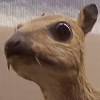
\includegraphics[width=0.32\textwidth]{images/heatmap/scoiattolo1.png}
			\caption{\textit{Original}}
		\end{minipage}
		\hfill
		\begin{minipage}[b]{0.45\textwidth}
			\centering
			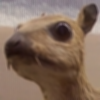
\includegraphics[width=0.32\textwidth]{images/heatmap/scoiattolo1_blur.png}
			\caption{\textit{Mean filtering 3x3}}
		\end{minipage}
	\end{figure}

	This solution can be exploited in order to make the pixels that suffers from the noise problem more smooth with the respect to the neighbors ones. In this way, even if the two consecutive frames are not exactly the same, the difference among the single pixels will be lower, resorting to a lower data sent over the socket. Let's take for simplicity two frames that are in gray scale, between 0 and 255, that are describes as two 3x3 matrices.
	\begin{center}
		$
		A = \frac{1}{9}\begin{bmatrix}
		120 & 131 & 112\\
			112 & 101 & 82\\
			44 & 106 & 65
		\end{bmatrix}
	\quad\quad B = \begin{bmatrix}
			120 & 139 & 90\\
			99 & 126 & 106\\
			46 & 75 & 88
		\end{bmatrix}
		$
	\end{center}
	If we simply compute the difference, and we set the threshold to 20, by computing the difference location by location, 5 pixels must be sent as difference. If we apply now the kernel to both the two frames, in order to simulate the behaviour of the algorithm, the two resulting matrices are the following:
	\begin{center}
		$
		A = \frac{1}{9}\begin{bmatrix}
			51 & 73 & 47\\
			68 & 96 & 66\\
			40 & 56 & 39
		\end{bmatrix}
		\quad\quad B = \begin{bmatrix}
			53 & 75 & 51\\
			67 & 98 & 69\\
			38 & 60 & 43
		\end{bmatrix}
		$
	\end{center}
	As you can see now, no pixels need to be sent. This is a huge improvement, since we have saved 100\% of the bandwidth if we neglect the overhead to transmit the information that no pixels have changed. Even if this seems an optimal solution, it has one major drawback. The image will became distorted from the details point of view. In fact, a trade-off between image quality and saved bandwidth must be selected.


	\subsection{Gaussian filter}
	The second type of filter that has been selected to reduce the noise, is the \textit{Gaussian filter}, that allows to reach a similar result with the respect to the Mean one. The idea is always to distorce the image to reduce the noise and make the difference among pixels lower. The matrix of a 3x3 Gaussian filter is the following:
		\begin{center}
		$
		K = \frac{1}{16}\begin{bmatrix}
			1 & 2 & 1\\
			2 & 4 & 2\\
			1 & 2 & 1
		\end{bmatrix}
		$
	\end{center}
	It can be computed using the following formula:
	\begin{align*}
		K(x,y) = \frac{1}{2 \cdot \pi \cdot \sigma^2}\cdot e^{-\frac{x^2 + y^2}{2 \sigma^2}}
	\end{align*}
	It is called Gaussian filter because of its shape, corresponds to a Gaussian function. A filter of this type requires $6 \sigma - 1$ values (to make it sure it's odd), so that for a $\sigma$ of 3 the kernel must be 17 elements long. The $\sigma$ value if given is pixels. If we use a square kernel its size can be simply computed as:
	\[
		side_{lenght} = \sqrt{6 \cdot \sigma - 1}
	\]
	Where $side_{lenght}$ is one of the length of the matrix that composes the kernel. A visual example representation is available in the following image.
	\begin{center}
		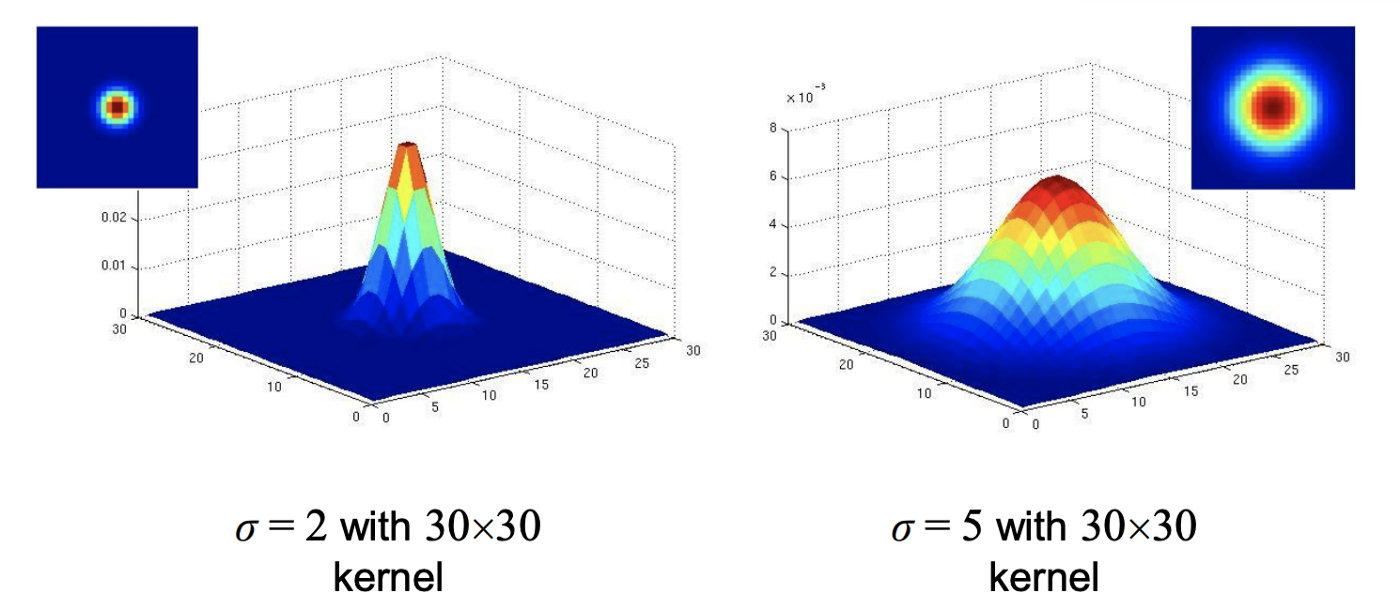
\includegraphics[width=0.45\linewidth]{images/heatmap/sigma_representation}
	\end{center}
	Gaussian filter weights pixels into a bell-shape curve around the central pixel. This means that the farther the pixel from the center, the lower the weight. On the other hand the Mean filter is just an average between the center and the neighboring pixels. This means that that for all the pixels, equal weights are assigned, regardless the distance from the center.
		\begin{figure}[H]
		\centering
		\begin{minipage}[b]{0.45\textwidth}
			\centering
			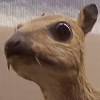
\includegraphics[width=0.32\textwidth]{images/heatmap/scoiattolo1.png}
			\caption{\textit{Original}}
		\end{minipage}
		\hfill
		\begin{minipage}[b]{0.45\textwidth}
			\centering
			
\includegraphics[width=0.32\textwidth]{images/heatmap/scoiattolo1_gaussian.png}
			\caption{\textit{Gaussian filter 3x3}}
		\end{minipage}
	\end{figure}

	The C code, that give $\sigma$, computes the entire convolution matrix is the following:
\begin{lstlisting}[style=CStyle]
float* computeGaussianKernel(float s, int K){
	float sum = 0;
	float* k = (float*)malloc(K*K*sizeof(float));
	for (int i = 0; i < K; i++){
		for (int j = 0; j < K; j++){
			double x = i - (K - 1) / 2.0;
			double y = j - (K - 1) / 2.0;
			k[i*K+j] = (1.0/(2.0*M_PI*s*s)) * exp(-((x*x + y*y)/(2.0*s*s)));
			sum += k[i*K+j];
		}
	}
	for (int i = 0; i < K; i++) {
		for (int j = 0; j < K; j++) {
			k[i*K+j] /= sum;
		}
	}
	
	return k;
}\end{lstlisting}	

	\subsection{CUDA implementation}
	In order to test the effectiveness of the algorithm and if it is suitable for this project, a configurable implementation has been developed in CUDA. In order to have all the same test environment, two sequential frames have been taken from the webcam in a semi dark environment with a person in the center. 
	
	\begin{figure}[H]
		\centering
		\begin{minipage}[b]{0.45\textwidth}
			\centering
			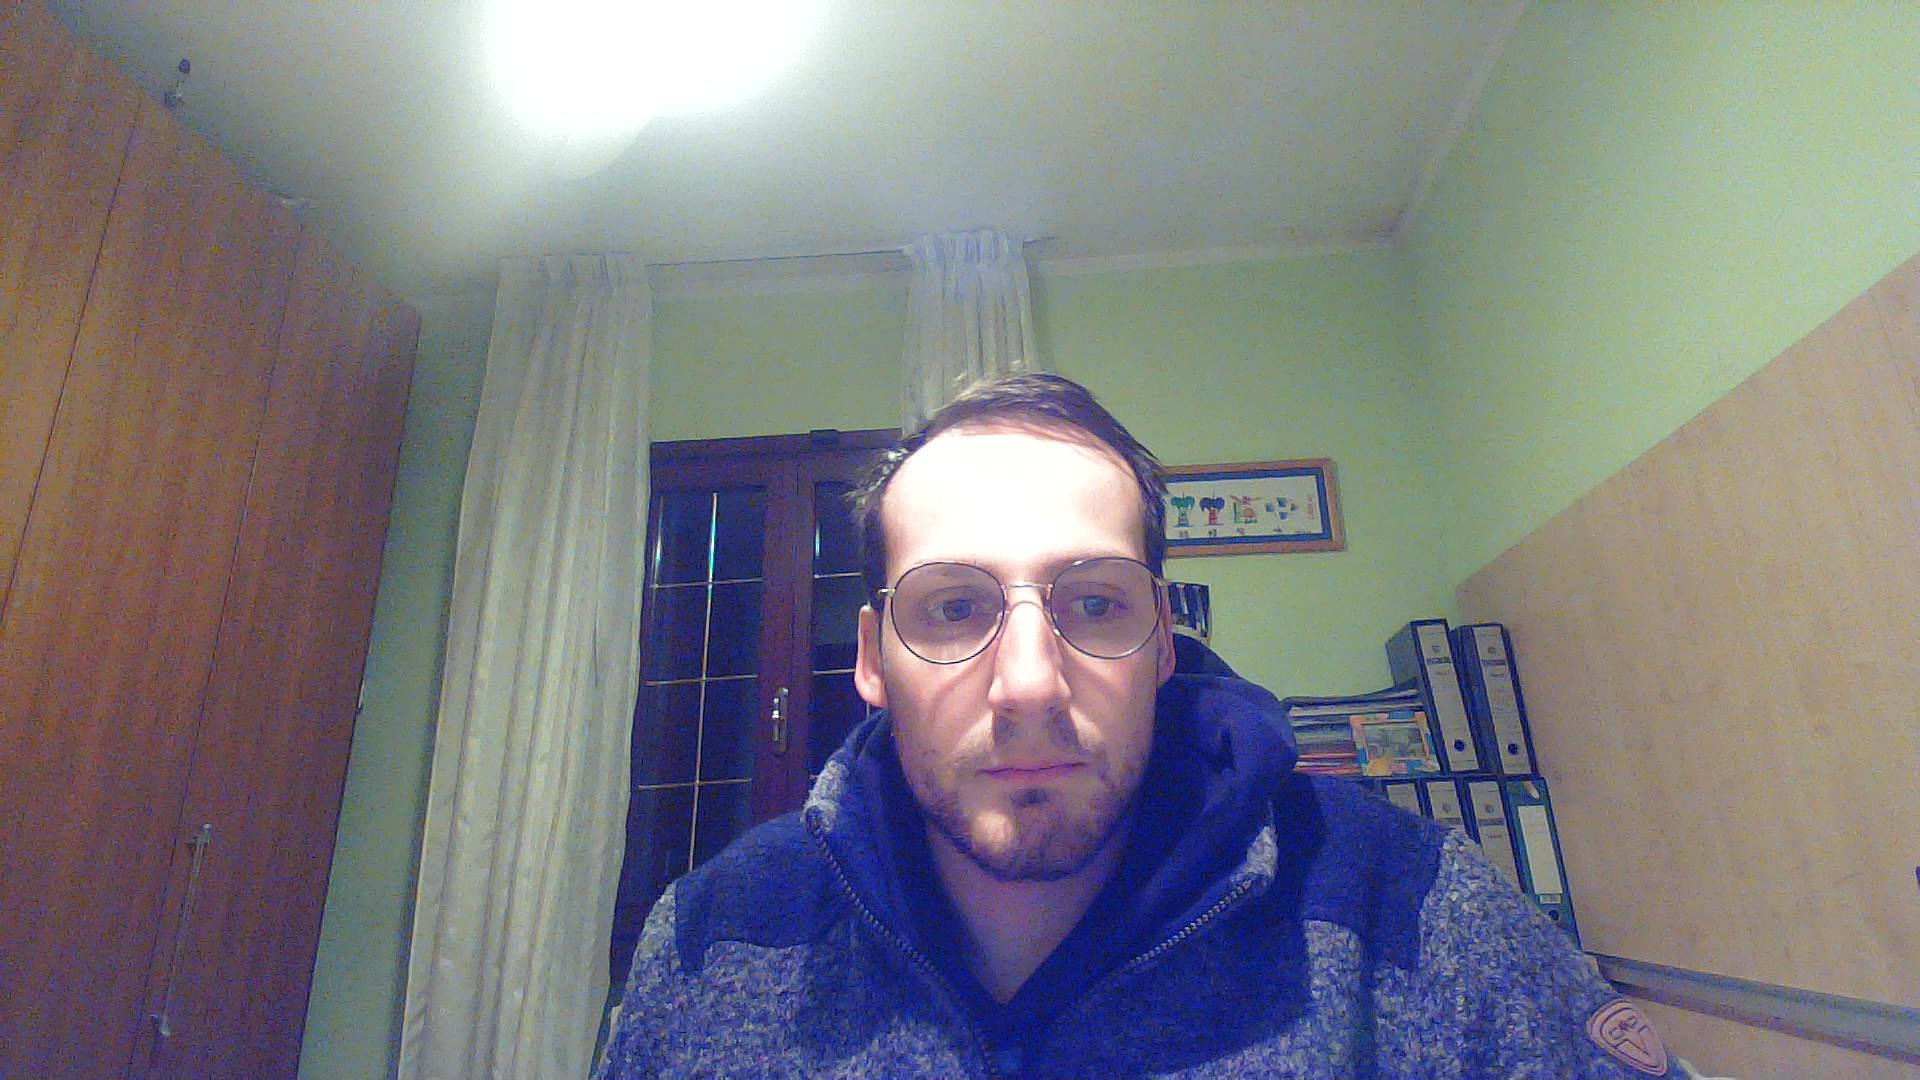
\includegraphics[width=0.85\textwidth]{images/heatmap/f1.jpg}
			\caption{\textit{First frame}}
		\end{minipage}
		\hfill
		\begin{minipage}[b]{0.45\textwidth}
			\centering
			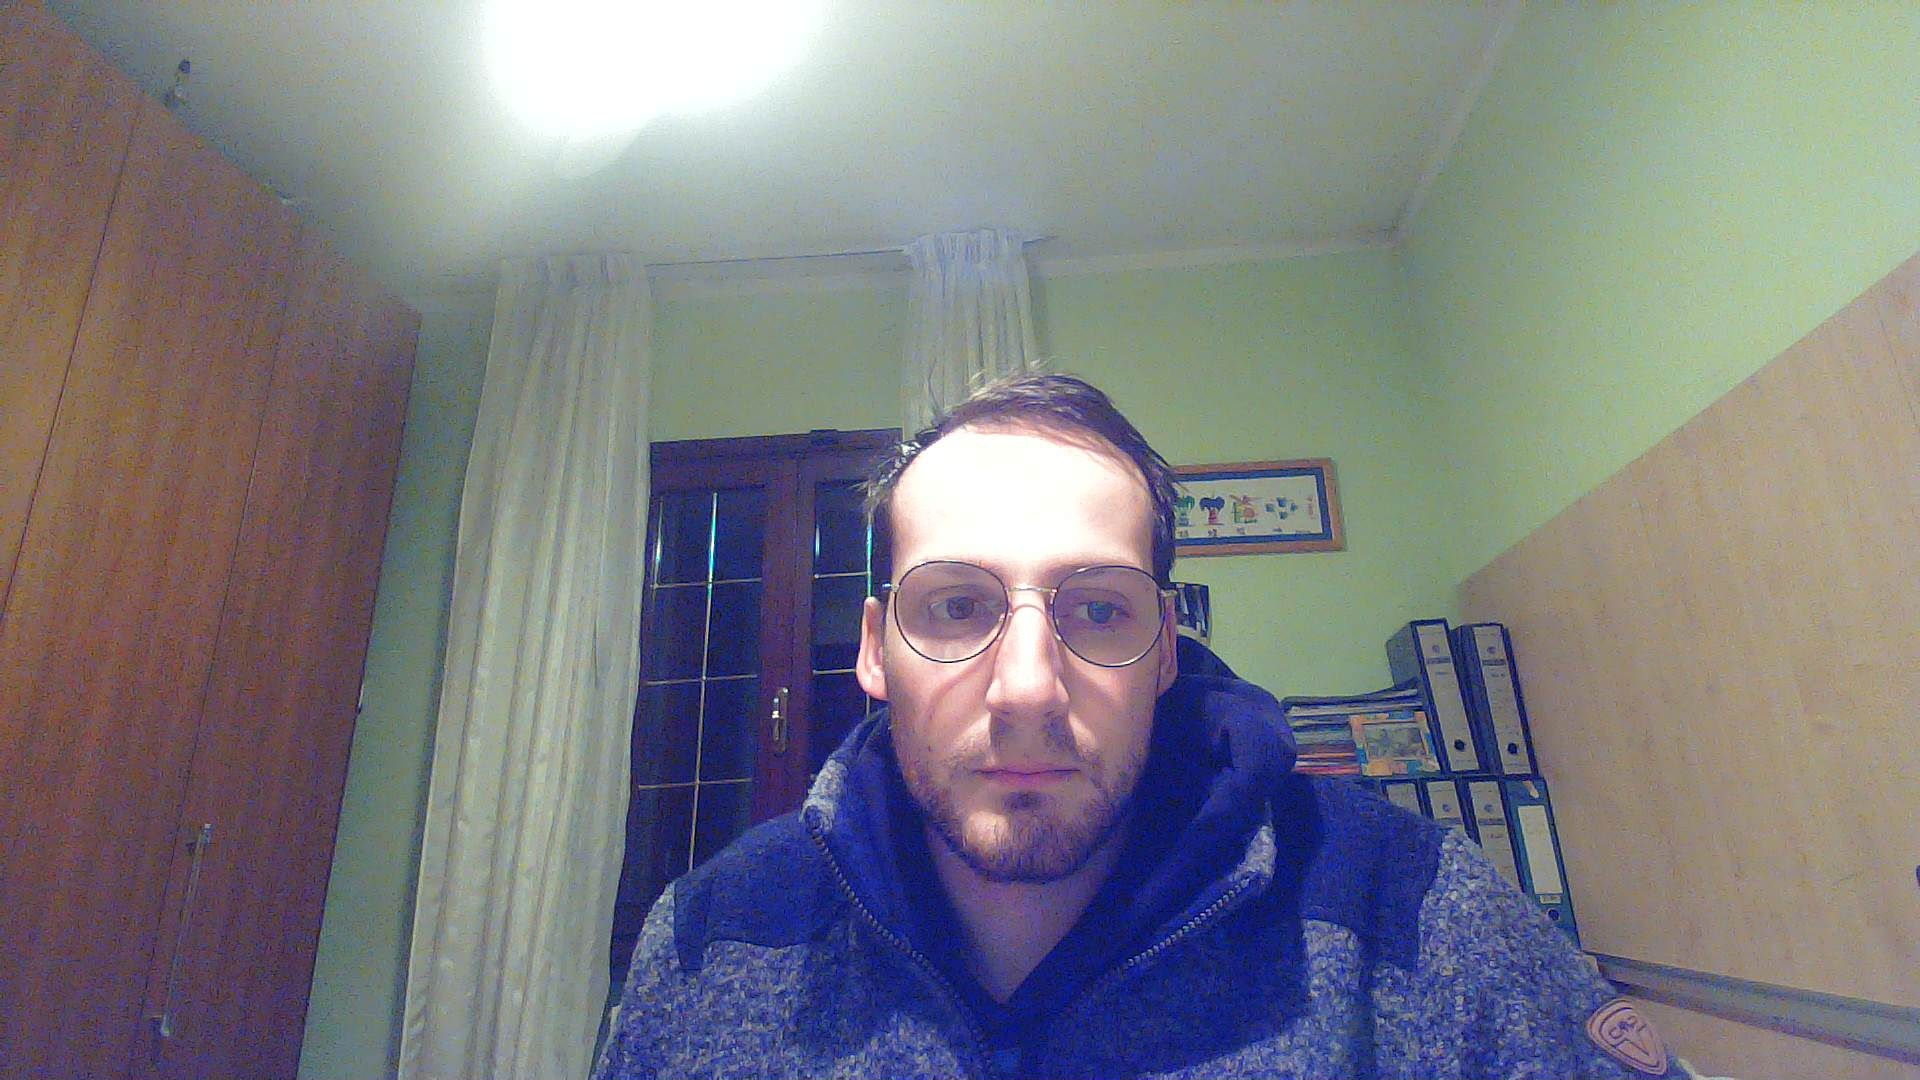
\includegraphics[width=0.85\textwidth]{images/heatmap/f2.jpg}
			\caption{\textit{Second frame}}
		\end{minipage}
	\end{figure}
	As you can see, the two images are pretty similar in term of content; a trained eye can see that the head of the second frame is slightly tilted to the right with the respect to the previous one. The idea is to run now the \textit{noise visualizer}, refer to Section \ref{sec:noise_visualizer}, on these two frames and understand where the noise is located.
	\begin{figure}[H]
		\centering
		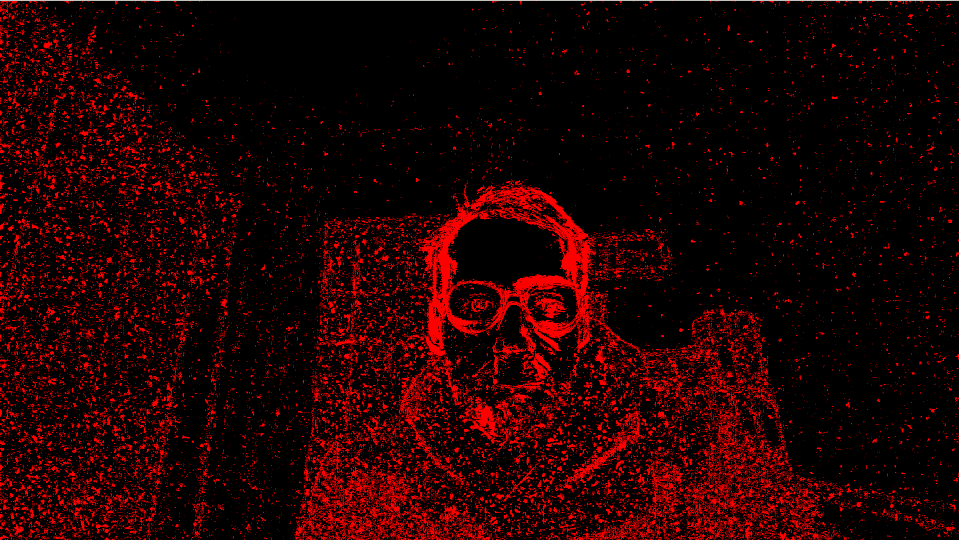
\includegraphics[width=0.35\linewidth]{images/heatmap/noise_visual}
		\caption{\textit{Red-black representation of the noise}}
		\label{fig:noisevisual}
	\end{figure}
	The noise, is the one in the background that do not contribute in any way to the video flow. In fact, even if it is fixed, it is sent anyway via the socket, increasing the used bandwidth. The CUDA implementation is based on the 2D tiled version but includes the management for all three color components.\newline\newline
	The entire algorithm is based on the usage of the shared memory and the synchronization among the thread. The idea is to make each thread work on single pixel and apply the kernel, by using the portion of the image that is in the shared memory, called \textit{tile}. 

	The kernel implementation is composed of multiple parts:
	\begin{enumerate}
		\itemsep0sp
		\item \textbf{Shared memory initialization and boundary condition management}:
		As introduced before, each thread, identified by its $ty$ and $tx$ coordinates should work on a precise pixels, identified as:
		\begin{lstlisting}[style=CStyle]
__shared__ int N_ds[BLOCK_SIZE][BLOCK_SIZE*3];

x = threadIdx.x + blockIdx.x*TILE_SIZE - K/2;
y = threadIdx.y + blockIdx.y*TILE_SIZE - K/2; \end{lstlisting}
	In fact, the idea is to create a block of threads that corresponds to \texttt{BLOCK\_SIZE}*\texttt{BLOCK\_SIZE} as dimension, so that each one of the loads into the shared memory the value of its pixel (the multiplication by 3 in the kernel implies that each threads read all three color components). The following code, instead, includes also the write into the shared memory.
		
		\begin{lstlisting}[style=CStyle]
int tx = threadIdx.x;   //W
int ty = threadIdx.y;   //H
int row_o = blockIdx.y*TILE_SIZE + ty;
int col_o = blockIdx.x*TILE_SIZE + tx;
int row_i = row_o - K/2;
int col_i = col_o - K/2;

if(row_i >= 0 && row_i < H && col_i >= 0 && col_i < W){
	N_ds[ty][tx*3] = image[row_i*W*3+ col_i * C];
	N_ds[ty][tx*3+1] = image[row_i*W*3+ col_i*3 + 1 ];
	N_ds[ty][tx*3+2] = image[row_i*W*3+ col_i*3 + 2 ];
} else {
	N_ds[ty][tx*3] = 0;
	N_ds[ty][tx*3+1] = 0;
	N_ds[ty][tx*3+1] = 0;
}	\end{lstlisting}
	The value \texttt{TILE\_SIZE} defines the dimension of the tile, in which each the kernel is applied. The problem is that, the first pixel (position [0,0]) in the image, if the kernel has a dimension of 3x3, need to access also the location [-1,-1], [-1, 0], [-1, 1], [0, -1], [1, -1]. In this case, they are not available. This is the reason of the presence of the if condition, that sets 0 at these locations in the shared memory by ``shifting" the indexes by $K/2$. The problem is shown in the below picture:
		\begin{figure}[H]
			\centering
			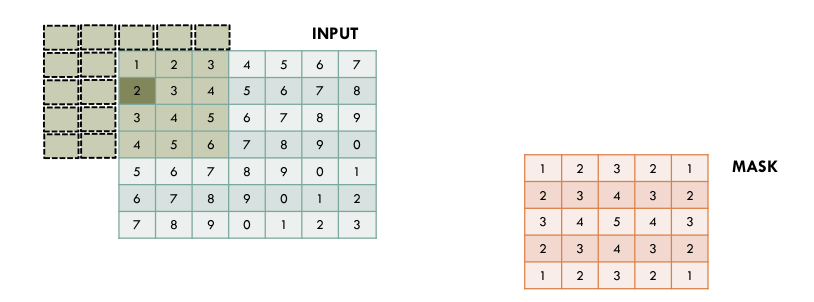
\includegraphics[width=0.45\linewidth]{images/heatmap/kernel_and_mask}
			\caption{\textit{Boundary conditions among the image border}}
			\label{fig:kernelandmask}
		\end{figure}
	In this way, all the pixels needed to process a tile of \texttt{TILE\_SIZE}x\texttt{TILE\_SIZE} dimension, are loaded into the \texttt{N\_ds} shared memory that is large \texttt{BLOCK\_SIZE}*\texttt{BLOCK\_SIZE*3} in order to contains also the values at the boundary of the tile.
		\item \textbf{Filter application}:
		Foreach element in the tile and for all three color components, the kernel is computed using the shared memory. 
	\end{enumerate}
	 


	The entire kernel is the following:

\begin{lstlisting}[style=CStyle]
__constant__ float dev_k[K*K];

__global__ void convolution_kernel(uint8_t *image, uint8_t *R)
{
	__shared__ int N_ds[BLOCK_SIZE][BLOCK_SIZE*3];
	
	int tx = threadIdx.x;   //W
	int ty = threadIdx.y;   //H
	int row_o = blockIdx.y*TILE_SIZE + ty;
	int col_o = blockIdx.x*TILE_SIZE + tx;
	int row_i = row_o - K/2;
	int col_i = col_o - K/2;
	
	// Management of the boudary conditions
	if(row_i >= 0 && row_i < H && col_i >= 0 && col_i < W){
		N_ds[ty][tx*3] = image[row_i*W*3+ col_i * C];
		N_ds[ty][tx*3+1] = image[row_i*W*3+ col_i*3 + 1 ];
		N_ds[ty][tx*3+2] = image[row_i*W*3+ col_i*3 + 2 ];
	} else {
		N_ds[ty][tx*3] = 0;
		N_ds[ty][tx*3+1] = 0;
		N_ds[ty][tx*3+1] = 0;
	}
	
    __syncthreads();

	if(row_o < H && col_o < W){
		float outputR = 0.0;
		float outputG = 0.0;
		float outputB = 0.0;
		if(ty < TILE_SIZE && tx < TILE_SIZE){
			for(int i = 0; i < K; i++)
			for(int j = 0; j < K; j++){
				outputR += dev_k[i*K+j] * N_ds[i+ty][(j+tx)*3];
				outputG += dev_k[i*K+j] * N_ds[i+ty][(j+tx)*3 + 1];
				outputB += dev_k[i*K+j] * N_ds[i+ty][(j+tx)*3 +2];
			}
			
			R[row_o*W*3 + col_o*3] = outputR;
			R[row_o*W*3 + col_o*3 + 1] = outputG;
			R[row_o*W*3 + col_o*3 + 2] = outputB;
		}
	}
}\end{lstlisting}

	The kernel call needs to work on an image of 1920*1080*3 elements divided into square tiles of \texttt{TILE\_SIZE}x\texttt{TILE\_SIZE} dimensions. Since the tile needs also the surrounding element to compute the kernel, the block size is composed of \texttt{BLOCK\_SIZE}x\texttt{BLOCK\_SIZE} elements, where:
	\[
		BLOCK\_SIZE = TILE\_SIZE + K - 1
	\]
	
	The grid instead, is configured to generate as many tile as needed from the image. In this case, a grid of \texttt{W/TILE\_SIZE}x\texttt{H/TILE\_SIZE} is enough (need to be rounded to the upper value).
	This is the complete kernel call
\begin{lstlisting}[style=CStyle]
dim3 blockSize, gridSize;
blockSize.x = BLOCK_SIZE, blockSize.y = BLOCK_SIZE, blockSize.z = 1;
gridSize.x = ceil((float)W/TILE_SIZE),
gridSize.y = ceil((float)H/TILE_SIZE),
gridSize.z = 1;

// Kernel call
convolution_kernel<<<gridSize, blockSize>>>(d_current, d_current_filtered);
\end{lstlisting}

	 This solution includes already optimal solution in order to increase the performance and reduce at minimum the overhead introduced by the computation of the filter. In fact, by having defined how convolution if performed, it can be simple called, after have set the kernel in the constant memory.
	 
	 Having defined the kernel, that once computed is fixed for the entire program execution, allows to not cope with the cache coherence management, allowing data to be aggressively cached in the L1 cache (the nearest to the SM).
	
	Moreover, access to the memory has been optimized by resorting to the usage of the shared memory. Since the larger the dimension of the tile, the higher the ration between the manipulated pixels and the memory accesses, an optimal solution is to increase as much as possible the tile size. The limit is the shared memory, that is limited. \newline\newline
	The execution of the kernel is inversely proportional to the size of the tile and the kernel dimension; the code shown before has been run for multiple sessions in order to be able to plot the following data:

	\begin{figure}[H]
		\centering
		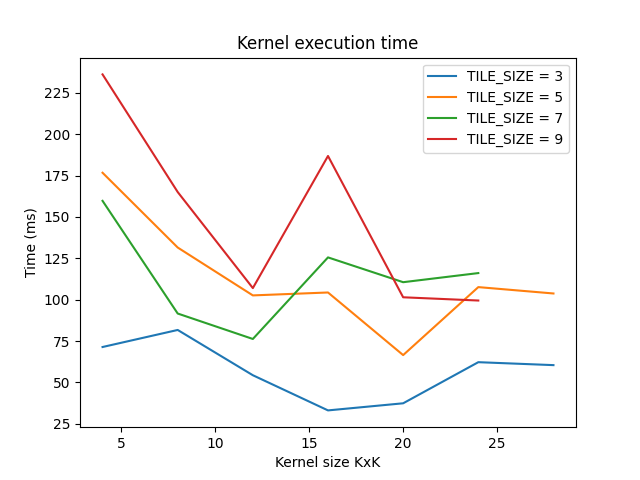
\includegraphics[width=0.42\linewidth]{images/heatmap/kernel_time_noise_2.png}
		\caption{\textit{Kernel execution time from profiler}}
		\label{fig:noise_kernel_time}
	\end{figure}

TODO:
	\begin{itemize}
		\item Try vertical and horizontal kernel
		\item try median and mean
		\item show new number of different pixels
	\end{itemize}
	
\end{document}
	